
%%%%%%%%%%%%%%%%%%%%%%%%%%%%%%%%%%%%%%%%%%%%%%%%%%%%%%%%%%%%%%%%%%%%%%%%%%
% AGN candidates figure                                                  %
%%%%%%%%%%%%%%%%%%%%%%%%%%%%%%%%%%%%%%%%%%%%%%%%%%%%%%%%%%%%%%%%%%%%%%%%%%

\begin{figure}[!b]
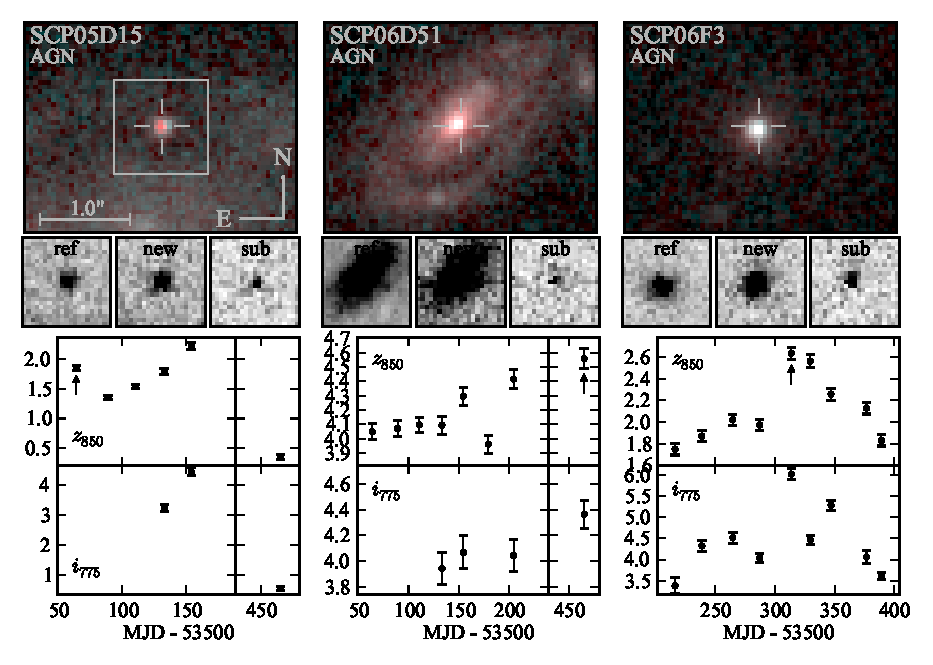
\includegraphics[width=\textwidth]{figures/cands/agn1.eps}
\caption[Images and light curves of candidates classified as AGN]
        {Images and light curves of the candidates classified as
          AGN. For each candidate, the \emph{top panel} shows the
          two-color stacked image ($i_{775}$ and $z_{850}$) of the
          host galaxy, with the position of the transient indicated.
          The \emph{three smaller panels} below the stacked image show the
          reference, new, and subtracted images for the discovery
          visit. The \emph{bottom panel} shows the light curve at the transient
          position (including host galaxy light) in the $z_{850}$
          ({\it top}) and $i_{775}$ ({\it bottom}) bands. The y axes
          have units of counts per second in a $3$~pixel radius
          aperture. The effective zeropoints are 23.94 and 25.02 for
          $z_{850}$ and $i_{775}$, respectively. The discovery visit
          is indicated with an arrow in the $z_{850}$
          plot. [\emph{Continued on next two pages.}]\label{fig:agn}}
\end{figure}

\begin{figure}[p]
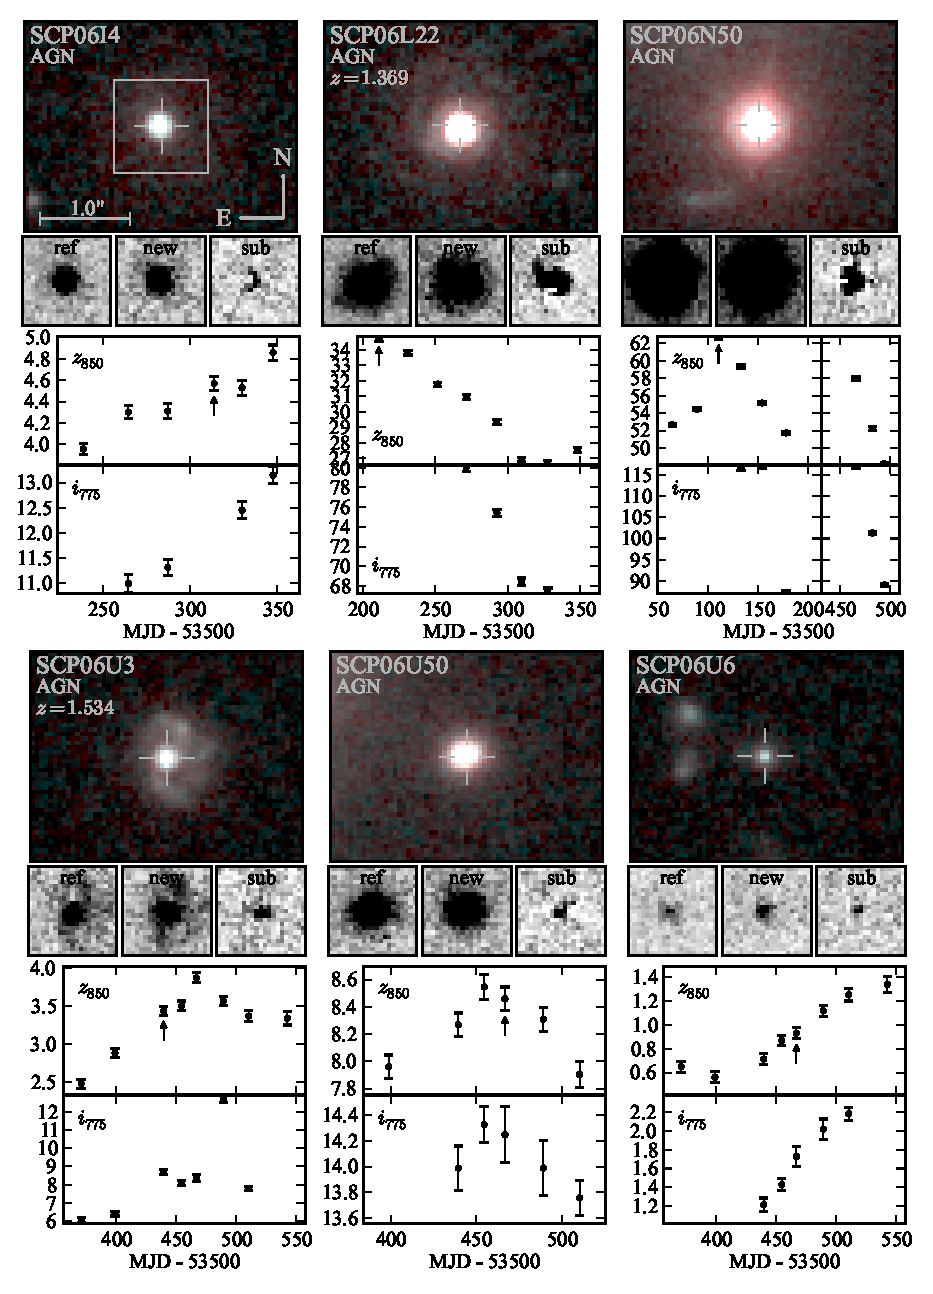
\includegraphics[width=\textwidth]{figures/cands/agn2.eps}
\end{figure}

\begin{figure}[p]
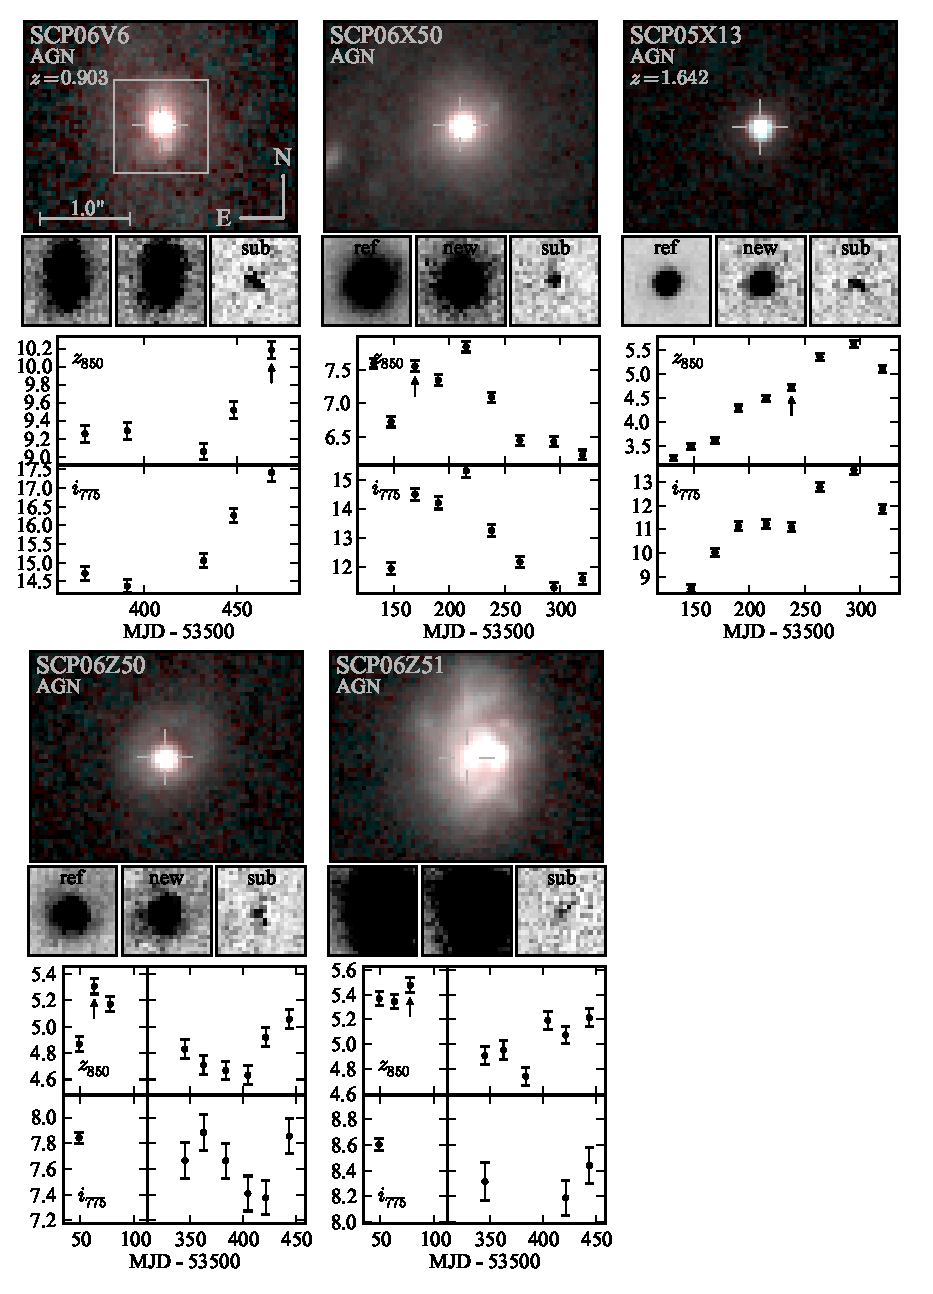
\includegraphics[width=\textwidth]{figures/cands/agn3.eps}
\end{figure}

Candidates positioned directly on the cores of their host galaxies may
be AGN. Four such candidates were spectroscopically confirmed as AGN:
SCP06L22 ($z=1.369$), SCP06V6 ($z=0.903$) and SCP05X13 ($z=1.642$) and
SCP06U3 ($z=1.534$). A fifth candidate, SCP06F3, is spectroscopically
consistent with an AGN at $z=1.21$, but is less certain \citep[see
  spectroscopy reported in][]{morokuma10a}. SCP06L22, SCP05X13,
SCP06U3 and SCP06F3 also have light curves that are clearly
inconsistent with SNe~Ia (observer frame rise times of 100~days or
more, or declining phases preceding rising phases; see
Fig.~\ref{fig:agn}). Of the ``on core'' candidates that were not
observed spectroscopically, five exhibit light curves that decline
before rising or have rise times of 100~days or more. A sixth
candidate, SCP06Z51 exhibited slightly varying fluxes that could be
due to either subtraction residuals or an AGN.  However, its light
curve is clearly inconsistent with a SN~Ia, especially considering the
apparent size, magnitude and color of the host galaxy. Summarizing,
there are 11 ``on-core'' candidates certain not to be SNe~Ia.

Three other ``on-core'' candidates are also considered likely AGN on
the basis of their light curves: SCP06Z50, SCP06U50 and
SCP06D51. SCP06Z50 has a rise-fall behavior in the first three
$z_{850}$ observations of its light curve that \emph{could} be
consistent with a SN~Ia light curve. However, given that the host
galaxy is likely at $z \lesssim 1$ based on its magnitude and color,
the SN would be fainter than a normal SN~Ia by 1~magnitude or
more. Considering the proximity to the galaxy core and the additional
variability seen in the last two observations, SCP06Z50 is most likely
an AGN. The light curve of candidate SCP06U50 also exhibits a
rise-fall that could be consistent with a supernova light
curve. However, its host is morphologically elliptical and likely at
$z \lesssim 0.7$ based on its color. At $z \lesssim 0.7$, a SN~Ia
would have to be very reddened ($E(B-V) \gtrsim 1$) to match the color
and magnitude of the SCP06U50 light curve. As this is very unlikely
(considering that the elliptical host likely contains little dust), we
conclude that SCP06U50 is also most likely an AGN. Finally, SCP06D51
was discovered in the last visit, on the core of a spiral galaxy. We
classify it as an AGN based on the earlier variability in the light
curve. As these galaxies are all most likely in the cluster
foregrounds, even the small uncertainty in these classifications is
not a concern for the cluster rate calculation here.

Note that one of the candidates classified here as a clear AGN,
SCP06U6, was reported as a SN with unknown redshift by
\citet{dawson09a}, due to the fact that spectroscopy revealed no
evidence of an AGN.  However, it is on the core of a compact galaxy,
and has a clear $\gtrsim 100$ day rise in both $z_{850}$ and
$i_{775}$. While it could possibly be a very peculiar SN with a long
rise time, what is important for this analysis is that it is clearly
not a SN~Ia.

